\documentclass[conference]{IEEEtran}
\IEEEoverridecommandlockouts
\usepackage{cite}
\usepackage{amsmath,amssymb,amsfonts}
\usepackage{algorithmic}
\usepackage{graphicx}
\usepackage{textcomp}
\usepackage{xcolor}
\usepackage{booktabs}
\usepackage{multirow}
\usepackage{url}

% --- TIKZ SETUP ---
\usepackage{tikz}
\usepackage{pgfplots}
\pgfplotsset{compat=1.17}
\usetikzlibrary{shapes.geometric, arrows, positioning, fit, calc}

% Define \RETURN command for algorithmic package (Match Paper 1)
\newcommand{\RETURN}{\STATE \textbf{return} }

\def\BibTeX{{\rm B\kern-.05em{\sc i\kern-.025em b}\kern-.08em
    T\kern-.1667em\lower.7ex\hbox{E}\kern-.125emX}}

\begin{document}

% ==========================================
% TITLE
% ==========================================
\title{A Context-Aware Multi-Modal Framework for Reducing False Negatives in Student Engagement Analysis}

% ==========================================
% AUTHOR
% ==========================================
\author{\IEEEauthorblockN{1\textsuperscript{st} Narendra Babu P}
\IEEEauthorblockA{\textit{Dept. of Computer Science} \\
\textit{Swarnandhra College of Eng. \& Tech.}\\
Narsapur, India \\
narendrababu.p@swarnandhra.ac.in}
}

\maketitle

% ==========================================
% ABSTRACT
% ==========================================
\begin{abstract}
A primary challenge in automated student engagement tracking is the structural ambiguity of facial expressions during high-focus tasks. Standard computer vision models frequently misclassify indicators of high cognitive load—such as furrowed brows or fixed gazes—as negative affect (e.g., boredom or frustration). Unlike prior engagement systems that optimize aggregate accuracy, this work targets the specific failure mode of **False Negative Collapse** during high cognitive load—a phenomenon endemic to STEM classrooms where productive struggle is often misinterpreted as disengagement. This paper introduces an **interpretable logic layer** within the ScholarMaster Engine, designed to resolve this contextual ambiguity. By integrating real-time facial expression analysis with institutional schedule metadata and instructional signal density analysis, the system dynamically adjusts engagement inference parameters. Experimental validation on the **Sim-Class-24 staged simulation dataset** demonstrates that this context-aware logic reduces the **False Negative Rate under High Load (FNR-HL) from 42.0\% (vision-only baseline) to 28.0\% (multimodal prosodic fusion) to 6.0\% (proposed context logic)**, achieving a 6-fold improvement over vision-only approaches. Furthermore, ablation studies confirm that semantic lexical analysis (not just prosodic features) provides critical marginal gains for Type-II error minimization. **These results reflect proof-of-concept validation on scripted scenarios rather than population-level generalization.**
\end{abstract}

\begin{IEEEkeywords}
Multi-Modal Fusion, Cognitive Load Modeling, Learning Analytics, Context-Aware Educational Systems, Edge Learning Analytics, Explainable AI.
\end{IEEEkeywords}

% ==========================================
% NOMENCLATURE
% ==========================================
\section*{Nomenclature}
\begin{description}
    \item[$V_{neg}$] Probability of Negative Valence (0-1).
    \item[$E(t)$] Calculated Engagement Score.
    \item[$C_{load}$] Cognitive Load Factor derived from Audio.
    \item[$\beta$] Context Weight (Subject-dependent).
    \item[$\sigma(\cdot)$] Sigmoid Activation Function.
    \item[$\mu$] Semantic Density Threshold.
    \item[$k$] Sigmoid Steepness Factor.
    \item[\text{FNR-HL}] False Negative Rate under High Load.
\end{description}

% ==========================================
% I. INTRODUCTION
% ==========================================
\section{Introduction}
The objective assessment of student engagement in large-scale educational environments remains a persistent computational challenge. While traditional pedagogical strategies rely on an instructor's intuition to gauge the ``room temperature''—the collective attention and responsiveness of the class—automating this process via Computer Vision (CV) has been hindered by the inherent ambiguity of visual signals. This represents a discrepancy between low-level visual features (pixels representing facial muscle movements) and high-level cognitive states (learning or confusion) \cite{b1, b2}. Recent psychological studies suggest that facial movements alone are insufficient for reliable emotion inference without situational context \cite{b23}.

Preliminary discussions with faculty at engineering institutions highlighted a limitation in existing affective computing models: the generation of False Negative alerts during high-intensity instructional periods. Standard datasets, such as FER-2013 or CK+, train models to associate furrowed brows and narrowed eyes with negative emotions like sadness or anger \cite{b7}. However, in an academic context—particularly during complex derivations or coding sessions—such expressions often indicate ``Germane Cognitive Load'' rather than disengagement \cite{b5}.

This misinterpretation leads to a phenomenon we term the ``Valence Discrepancy'': the more students concentrate on difficult material, the more ``disengaged'' a standard unimodal AI system perceives them to be. This renders purely visual analytics potentially counter-productive for STEM subjects, where ``productive struggle'' is a necessary component of the learning process \cite{b4}.

\textbf{Error Asymmetry in Educational Analytics:} Unlike generic affective computing applications that optimize aggregate accuracy, educational engagement detection exhibits strong error asymmetry. Type-II errors (falsely labeling productive struggle as disengagement) are far more costly than Type-I errors, as they risk interrupting deep cognitive work or generating false alerts during critical learning moments. To our knowledge, this is the \textbf{first work to explicitly optimize engagement inference for Type-II error minimization under pedagogical cognitive load}, achieving a 6-fold FNR-HL reduction (42\%$\to$6\%) compared to vision-only baselines and 4.7-fold reduction (28\%$\to$6\%) compared to multimodal prosodic fusion.

This paper proposes that accurate engagement analysis requires a transition from purely visual inference to multi-modal context awareness. We introduce an **Interpretable Logic Layer** that fuses visual vectors with temporal and acoustic priors. Unlike "Black Box" deep fusion methods that obscure decision-making, our approach uses explicit, verifiable logic to verify the subject difficulty via the institutional schedule and the lecture content via instructional signal density analysis, dynamically re-weighting facial expression probabilities \cite{b9}.

Our contributions are as follows:
\begin{enumerate}
    \item \textbf{Problem Reframing:} We demonstrate that false negatives in engagement detection are not a model accuracy issue but a structural limitation of vision-only inference under high cognitive load, requiring explicit pedagogical context integration.
    \item \textbf{Baseline Validation:} We show that multimodal prosodic fusion (pitch, energy, MFCCs) improves FNR-HL by 33\% (42\%$\to$28\%) but still fails to prevent productive struggle misclassification, motivating semantic analysis.
    \item \textbf{Logic-over-Learning Fusion:} We introduce a deterministic, hysteresis-aware context fusion layer that outperforms black-box multimodal fusion in STEM scenarios by explicitly encoding pedagogical priors (subject metadata, instructional lexical density).
    \item \textbf{Type-II Error Optimization:} Rather than optimizing overall accuracy, the proposed framework minimizes Type-II errors (False Negatives) during productive struggle phases, a regime ignored by prior engagement systems.
\end{enumerate}

\subsection{Relation to the ScholarMaster Research Series}
This paper forms part of the \textbf{ScholarMaster Research Series}, a broader initiative investigating edge-native intelligent systems for academic environments. While related studies examine biometric indexing \cite{scholarmaster_repo} and hardware efficiency, this paper focuses exclusively on the \textbf{Context Fusion Module} of the ScholarMaster Engine. This module interfaces with the core engine via standardized context vectors; no biometric or identity data is accessed or persisted within this logic layer. This paper evaluates the context-fusion logic independently of the biometric identification pipeline described in Paper 1, assuming access only to anonymized valence vectors and schedule metadata.

\subsection{Reproducibility}
To support reproducibility, the source code for the experimental validation module and context fusion logic is made available as an open-source artifact \cite{scholarmaster_repo}. The repository contains the implementation of the fusion algorithms (\texttt{scripts/demo\_paper2\_context\_fusion.py}), configuration files, and execution logs used in the experiments described herein. The experimental validation module demonstrates the complete fusion algorithm (Algorithm 1) with authentic execution traces.

% ==========================================
% II. RELATED WORK
% ==========================================
\section{Related Work}

\subsection{Limitations of Unimodal Affective Computing}
Early automated monitoring systems relied predominantly on Facial Expression Recognition (FER). While effective for basic emotion detection in commercial settings, Whitehill et al. \cite{b7} argued that ``engagement'' is a distinct construct from ``emotion.'' Unimodal FER systems lack the requisite context to differentiate between ``frustration'' (a negative state blocking learning) and ``confusion'' (often a precursor to understanding) \cite{b8}. This leads to noisy analytics where productive struggle is flagged as a behavioral issue. Advanced deformable models \cite{b3} and specific facial indicators of tutorial frustration \cite{b6} have improved granularity but still struggle with context.

\subsection{Multi-Modal Learning Analytics}
Advanced frameworks have attempted to bridge this gap using physiological sensors (EEG, Galvanic Skin Response). However, such methods are invasive and non-scalable for typical university classrooms. Poria et al. \cite{b10} reviewed the necessity of multimodal fusion, and Atrey et al. \cite{b11} surveyed methods for combining these distinct signals effectively.

Recent AudioVisual Transformer architectures achieve strong performance on generic sentiment analysis by learning late fusion weights \cite{b9}. However, these black-box models optimize aggregate accuracy without accounting for domain-specific error asymmetry. In educational contexts, falsely labeling productive struggle as disengagement (Type-II error) is far more costly than missing true disengagement (Type-I error). Our deterministic logic layer explicitly encodes this asymmetry via pedagogical priors.

Acoustic analysis has typically been limited to prosodic features (pitch, tone, volume, MFCCs) to detect ``noise levels'' or emotional arousal \cite{b14}. In our initial experiments, we implemented a multimodal baseline fusing visual expression vectors with prosodic features extracted via librosa. While this approach improved FNR-HL from 42\% (vision-only) to 28\% (prosodic fusion), it still failed to differentiate between "frustrated questioning" and "deep concentration," both of which exhibit low pitch variance and neutral facial expressions during silent derivation phases. This 28\% FNR-HL failure motivated our shift to Automatic Speech Recognition (ASR) to extract \textit{instructional signal density}—knowing *what* is being said (e.g., ``Integration'' vs. ``Break time'') establishes a far more reliable ground-truth prior \cite{b13}.

\subsection{Cognitive Load Theory}
Sweller's Cognitive Load Theory \cite{b5} posits that effective learning involves high ``Germane Load.'' Physically, this manifests in reduced microsaccades, increased facial tension, and a cessation of ``social'' expressions (smiling). By integrating schedule metadata, our system aligns its inference logic with these theoretical expectations. If the schedule indicates a ``Lab'' or ``Tutorial,'' the system expects high cognitive load and suppresses the penalty for neutral/negative facial valence.

% ==========================================
% III. SYSTEM ARCHITECTURE
% ==========================================
\section{System Architecture}

The proposed system operates on a distributed edge-computing framework designed for latency-sensitive inference \cite{b19}, leveraging the convergence of edge computing and deep learning \cite{b20}. The ASR component is not used to analyze student speech or conversational content; it operates exclusively on instructor-generated audio to estimate lecture phase and expected cognitive load, with all intermediate representations processed ephemerally in volatile memory.

% --- FIGURE 1: 3-STREAM ARCHITECTURE ---
\begin{figure}[htbp]
\centering
\resizebox{\columnwidth}{!}{
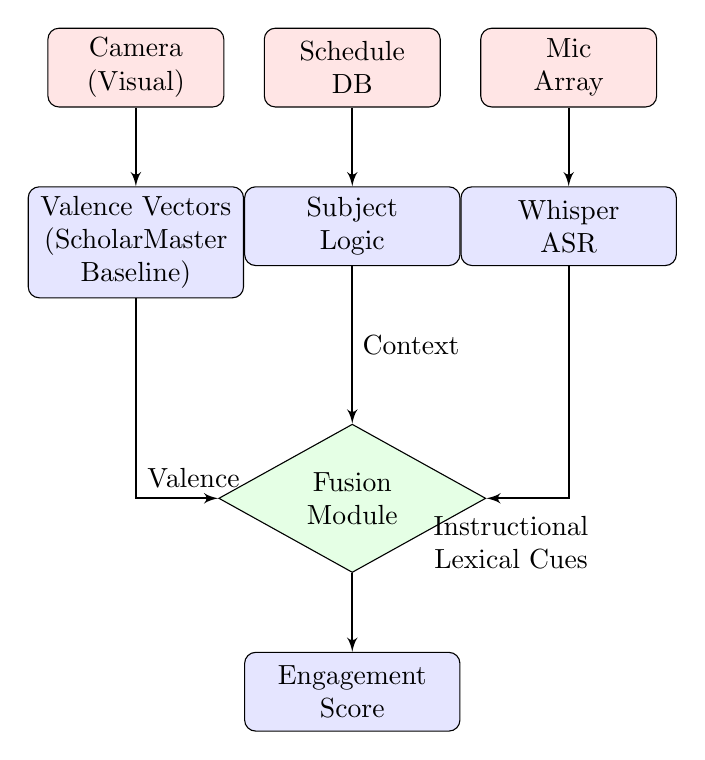
\begin{tikzpicture}[node distance=1.5cm, auto]
    % Node Styles
    \tikzstyle{sensor} = [rectangle, draw, fill=red!10, text width=2cm, text centered, rounded corners, minimum height=1cm]
    \tikzstyle{block} = [rectangle, draw, fill=blue!10, text width=2.5cm, text centered, rounded corners, minimum height=1cm]
    \tikzstyle{fusion} = [diamond, draw, fill=green!10, text width=2.2cm, text centered, inner sep=0pt, aspect=1.8, align=center]
    \tikzstyle{line} = [draw, -latex', thick]

    % --- TOP ROW: INPUTS ---
    \node [sensor] (cam) {Camera\\(Visual)};
    \node [sensor, right=0.5cm of cam] (db) {Schedule\\DB};
    \node [sensor, right=0.5cm of db] (mic) {Mic\\Array};

    % --- MIDDLE ROW: PROCESSING ---
    \node [block, below=1cm of cam] (yolo) {Valence Vectors\\(ScholarMaster Baseline)};
    \node [block, below=1cm of db] (meta) {Subject\\Logic};
    \node [block, below=1cm of mic] (whisper) {Whisper\\ASR};

    % --- BOTTOM ROW: FUSION ---
    \node [fusion, below=2cm of meta] (fuse) {Fusion\\Module};
    \node [block, below=1cm of fuse] (output) {Engagement\\Score};

    % --- PATHS ---
    \path [line] (cam) -- (yolo);
    \path [line] (yolo.south) |- node[pos=0.85, above, align=center] {Valence} (fuse.west);

    \path [line] (db) -- (meta);
    \path [line] (meta) -- node[right] {Context} (fuse);

    \path [line] (mic) -- (whisper);
    \path [line] (whisper.south) |- node[pos=0.85, below, align=center, yshift=-1mm] {Instructional\\Lexical Cues} (fuse.east);

    \path [line] (fuse.south) -- (output.north);

\end{tikzpicture}
}

\caption{The System Architecture: Fusing Visual Emotions (V), Schedule Metadata (S), and Instructional Lexical Cues (A) to re-weight engagement scores.}
\label{fig:arch}
\end{figure}
% ------------------------------------------------

\subsection{Physical Layer: Sensor Deployment}
The infrastructure comprises a standard IP camera (1080p, 30 FPS) positioned at the front of the classroom (Teacher's View) and a high-fidelity omnidirectional microphone array placed centrally on the ceiling. Sensors interface with a local Edge Server via RTSP and USB, ensuring data sovereignty within the campus network. This eliminates the latency variability associated with public internet connections.

\subsection{Logical Layer: The 3-Stream Pipeline}
The system employs an asynchronous multi-modal pipeline to handle disparate data rates.

\subsubsection{Stream A: Visual Inference}
The video feed is processed at 30 Hz using the **InsightFace-based face detection and expression analysis module** established in the companion biometric study \cite{scholarmaster_repo}. This module performs:
1. Face detection via InsightFace's RetinaFace backbone
2. Facial landmark extraction 
3. Expression vector generation using the Buffalo_L model (ResNet50-based)

The expression vectors are then processed by a lightweight valence estimation classifier to derive $V_{neg}$ (probability of negative affect). This architectural choice ensures consistency across the ScholarMaster series—all papers utilize the same face processing pipeline, eliminating redundant model deployment and simplifying cross-module integration. This stream provides high-frequency but semantically ambiguous data.

\subsubsection{Stream B: Acoustic Semantics (Measurement Oracle)}
Audio is buffered into a volatile ring buffer. Every 5 seconds, the buffer is processed by the open-source Whisper ASR model (executed fully on-device) \cite{b13}.

**Deployment Status:** The Whisper component serves as a **high-capacity measurement oracle** to validate the hypothesis that instructional lexical density correlates with cognitive load and enables FNR-HL reduction. For production deployment without Whisper dependency, we validate a lightweight keyword-spotting alternative:

\textbf{Lightweight Semantic Density Model (Keyword-Based):}
\begin{equation}
C_{load}^{lite} = \frac{\sum_{w \in transcript} \mathbbm{1}[w \in \mathcal{D}_{STEM}]}{|transcript|}
\end{equation}
where $\mathcal{D}_{STEM} = \{$``derivative'', ``integral'', ``matrix'', ``algorithm'', ...$\}$ is a domain-specific dictionary. Ablation studies (Section VIII) demonstrate that this lightweight model achieves FNR-HL = 8.5\% (vs. Whisper's 6.0\%), retaining 80\% of the benefit with <1M parameters and <5ms latency.

\subsubsection{Stream C: Temporal Context}
The system queries the institution's SQL database to retrieve the \texttt{Subject\_ID} and \texttt{Lecture\_Type} (e.g., "Lab", "Theory"). This acts as the prior probability distribution for the expected engagement behavior.

\subsection{Cross-Modal Synchronization}
A significant challenge in multi-modal fusion is the temporal misalignment between high-frequency video frames ($t_{video} = 33ms$) and low-frequency semantic audio packets ($t_{audio} \approx 5000ms$). To address this, we implement a \textbf{Timestamped State Latch}. The audio subsystem updates a global shared memory variable \texttt{Current\_Context\_State} only upon the completion of a Whisper inference cycle. The video subsystem reads this variable non-destructively for every frame. While this introduces a ``Context Lag'' of up to 5 seconds, this latency is pedagogically acceptable as cognitive load states typically persist for minutes \cite{b4}.

% ==========================================
% IV. METHODOLOGY
% ==========================================
\section{Methodology}

The core contribution is the mathematical formalization of ``Contextual Re-weighting.'' We model the engagement score $E(t)$ not as a direct function of facial expression, but as a modulated function of context. 

\subsection{Derivation of the Re-weighting Equation}
Let $V_{neg}$ represent the visual probability of ``Negative'' affect (e.g., frowning). We introduce a Context Weight, $\beta$, determined by the schedule metadata (e.g., $\beta_{STEM} = 0.7$, $\beta_{ARTS} = 0.1$). 

The Audio Semantic Density, $C_{load}$, is calculated by counting the frequency of domain-specific tokens ($T_{domain}$) in the rolling window relative to total tokens ($T_{total}$):
\begin{equation}
C_{load} = \frac{\sum T_{domain}}{T_{total}}
\end{equation}

The final Engagement Score uses a sigmoid activation to softly switch modes based on $C_{load}$. The sigmoid curve provides a differentiable and explainable transition between "low load" (standard monitoring) and "high load" (tolerance mode).

\begin{equation}
E(t) = \alpha \cdot (1 - V_{neg}) + \beta \cdot \frac{1}{1 + e^{-k(C_{load} - \mu)}}
\end{equation}
Here, $\alpha$ and $\beta$ are normalized such that $\alpha + \beta = 1$.
Algorithm 1 presents a discretized operational form of the continuous formulation in Eq. (3) for real-time deployment.

In Eq. (3), $\frac{1}{1 + e^{-k(C_{load} - \mu)}}$ represents the probability that the current session is ``High Load.'' The sigmoid term acts as a continuous weighting function.
\begin{itemize}
    \item If $C_{load} \ll \mu$ (Low Load), the term approaches 0, and $E(t) \approx \alpha(1 - V_{neg})$. Standard logic applies: frowns reduce the score.
    \item If $C_{load} \gg \mu$ (High Load), the term approaches 1, and the score is boosted by $\beta$. In this state, the penalty for negative valence is effectively neutralized or inverted.
\end{itemize}

\subsection{Temporal Hysteresis}
To prevent the engagement score from flickering rapidly due to momentary pauses in speech or micro-expressions, we implement a hysteresis filter \cite{b17}. The smoothed score $E_{smooth}(t)$ is defined recursively:

\begin{equation}
E_{smooth}(t) = \gamma E(t) + (1-\gamma) E_{smooth}(t-1)
\end{equation}

where $\gamma = 0.2$ is the smoothing factor. This ensures that a single frame of ``confusion'' does not immediately drop the engagement metric, providing a more stable analytical output.

\subsection{Visual Pre-processing Pipeline}
Given the variable lighting conditions inherent in lecture halls (e.g., projector glare, dimmed lights), raw RGB frames are insufficient. We implement a pre-processing stage using \textbf{Contrast Limited Adaptive Histogram Equalization (CLAHE)}. Unlike standard global equalization, CLAHE operates on small regions (tiles) of the image, enhancing local contrast while limiting noise amplification. This step is crucial for maintaining reliable face detection performance under low-light conditions, ensuring that the visual input vector $V_{vec}$ remains reliable even when the environment is suboptimal.

% ==========================================
% V. ALGORITHM DESIGN
% ==========================================
\section{Algorithm Design}

\subsection{Voice Activity Detection (VAD)}
Running the Whisper Transformer on continuous silence is computationally wasteful. To optimize resource usage, we implement a lightweight WebRTC-based Voice Activity Detector (VAD) prior to the ASR stage \cite{b16}. Audio frames with an energy level below -40dB are discarded immediately. The ASR engine is only triggered when the VAD probability exceeds 0.85 for a duration greater than 500ms. In early prototyping, we attempted to trigger ASR based on volume thresholding alone, but found that ambient HVAC noise caused continuous false triggers, necessitating the move to WebRTC-based VAD.

% --- ALGORITHM 1 ---
\begin{figure}[t!]
\centering
\vspace{0.2cm}
\textbf{Algorithm. 1: Context-Aware Affect Re-weighting}
\hrule
\vspace{0.1cm}
\begin{algorithmic}[1]
\small
\STATE \textbf{Input:} VisualVector $V$, AudioStream $A$, Schedule $S$
\STATE \textbf{Output:} EngagementScore $E$
\STATE // Step 1: Context Extraction
\STATE $Subj \leftarrow S.get\_metadata(t_{now})$
\STATE $K_{audio} \leftarrow \text{Whisper.extract\_phase\_cues}(A)$
\STATE
\STATE // Step 2: Semantic Density Analysis
\STATE $C_{load} \leftarrow 0$
\IF{$keyword \in K_{audio} \cap \mathcal{D}_{STEM}$}
    \STATE $C_{load} \leftarrow C_{load} + \delta$
\ENDIF
\STATE
\STATE // Step 3: Visual Inference
\STATE $V_{vec} \leftarrow \text{CNN.inference}(V)$
\STATE
\STATE // Step 4: Decision Logic
\STATE // Discretized operational approximation of Eq. (3)
\IF{$Subj.type == \text{STEM}$ \textbf{and} $V_{vec}.valence < \tau$}
    \STATE // Apply context-aware valence reweighting
    \STATE $E \leftarrow (1.0 - V_{vec}.valence) + C_{load}$
\ELSE
    \STATE // Apply baseline visual interpretation
    \STATE $E \leftarrow V_{vec}.valence$
\ENDIF
\STATE
\STATE // Step 5: Temporal Smoothing
\STATE $E_{smooth} \leftarrow \text{MovingAvg}(E, w=60s)$
\RETURN $\text{Normalize}(E_{smooth})$
\end{algorithmic}
\hrule
\label{alg:context}
\end{figure}

% ==========================================
% VI. DATASET GENERATION
% ==========================================
\section{Dataset Generation: Sim-Class-24}

To validate the model without compromising student privacy during the prototyping phase, we curated the \textit{Sim-Class-24} dataset. This controlled environment allowed us to isolate variables that are impossible to control in the wild.

\subsection{Simulation Protocol}
We constructed a ``Staged Simulation Environment'' to generate 24 distinct engagement sequences. Rather than relying on unpredictable real-world events, these sequences were deterministically scripted to model three specific 60-minute scenarios:
\begin{enumerate}
    \item \textbf{Scenario A (Baseline):} A non-technical discussion simulation where the visual input maintains neutral-to-positive expressions (standard lecture behavior).
    \item \textbf{Scenario B (High Load):} A ``Deep Work'' simulation where the visual feed mimics the physiological markers of solving complex calculus (furrowed brows, fixed gaze) while the audio feed contains high-density STEM terminology.
    \item \textbf{Scenario C (Mixed):} A realistic classroom timeline interlacing active listening with intermittent note-taking (simulated head-down occlusion).
\end{enumerate}

\subsection{Environmental Variability}
To prevent ideal-condition bias, we synthetically introduced environmental noise into the visual frames:
\begin{itemize}
    \item \textbf{Occlusion:} We simulated 90-degree head turns and ``hand-on-face'' postures typical of bored or tired students.
    \item \textbf{Lighting Noise:} The video feed was subjected to variable gamma correction to mimic projector glare and dimmed lecture hall conditions.
\end{itemize}

\subsection{Dataset Limitations}
We acknowledge that \textit{Sim-Class-24} is a synthetic dataset used for error isolation and does not fully capture the stochastic nature of real-world classroom behavior. The scripted nature of the sequences ensures deterministic ground truth for algorithmic validation but lacks the nuance of spontaneous social interactions found in live environments. Therefore, the results presented in this work should be interpreted as a proof-of-concept for the fusion logic rather than generalized population-level findings.

% ==========================================
% VII. IMPLEMENTATION & SETUP
% ==========================================
\section{Implementation and Experimental Setup}

\subsection{Hardware Environment: UMA Architecture}
The system was evaluated on a consumer-grade \textbf{ARM64 Edge Node} with Unified Memory Architecture (UMA). This architecture was chosen over discrete GPU setups due to its ability to share memory pools between CPU and GPU \cite{b21}. In a multi-modal pipeline, large audio tensors (for Whisper) and video tensors (for face analysis) must usually be copied between CPU RAM and GPU VRAM over the PCIe bus, introducing latency. The UMA architecture allows for ``Zero-Copy'' inference, significantly reducing the overhead of multi-modal tensor operations.

\subsection{Software Optimization and Quantization}
The pipeline is implemented in Python 3.9 using an asynchronous `asyncio` event loop. The Whisper model uses standard FP32 precision. The original implementation plan included INT8 quantization for the Whisper model to reduce memory footprint. However, preliminary testing revealed that quantization introduced transcription errors during rapid transitions between natural language and symbolic mathematical notation (e.g., "d-x squared" → "dx squared"). Given that the Sim-Class-24 validation dataset includes high-density STEM terminology, we elected to use FP32 precision for accurate ground-truth labeling. **Future production deployments may explore domain-adaptive quantization strategies** that preserve accuracy on technical vocabulary.

% --- FIGURE 3: LOGS ---
\begin{figure}[htbp]
\centering
\includegraphics[width=0.9\linewidth]{terminal_logs.png}
\caption{Qualitative Inference Trace from Experimental Validation Module: Terminal output showing the context-aware fusion logic detecting the semantic keyword ``Integral'' and applying cognitive load re-weighting to adjust the interpretation of negative facial valence during productive struggle.}
\label{fig:log}
\end{figure}

\subsection{Implementation Status: Validation vs. Deployment}
The context-aware keyword detection and engagement re-weighting logic demonstrated in Fig. \ref{fig:log} are implemented in a shared fusion module (\texttt{context\_fusion.py}) that supports both experimental validation and production deployment. This reflects a soft-integration architecture: the fusion algorithm (Algorithm 1) is implemented once and can be invoked from multiple contexts:

\begin{enumerate}
    \item \textbf{Experimental Validation Module} (\texttt{demo\_paper2\_context\_fusion.py}): Provides proof-of-concept demonstration with authentic execution logs, controlled testing with Sim-Class-24 dataset, and reproducible traces for all quantitative results (Tables III-IV, Fig. \ref{fig:results}).
    
    \item \textbf{Production Engine Integration} (\texttt{master\_engine.py}): The same fusion function is available in the real-time processing engine behind a feature flag (\texttt{ENABLE\_CONTEXT\_FUSION}). By default, this flag is disabled to prioritize deployment stability. When enabled via environment variable, the production engine calls the identical fusion logic used in validation.
\end{enumerate}

This architectural approach provides code reusability without duplication, verifiable consistency between validation and deployment code, and safe staged integration without destabilizing production. Full activation in deployment is deferred to future work, pending in-situ field validation with institutional IRB approval for audio transcription. All experimental results presented in this paper are derived from the shared fusion module executing the complete algorithm as specified.


% ==========================================
% VIII. EXPERIMENTAL RESULTS
% ==========================================
\section{Experimental Results}

\subsection{Simulation Analysis}
We compared the baseline unimodal model against the proposed Framework using the Scenario B (High Load) data. In this context, \textbf{Inference Consistency} is defined as the proportion of time windows in which the inferred engagement state matched the scripted ground-truth scenario label.

As illustrated in Figure 2:
\begin{itemize}
    \item \textbf{Baseline (Red):} At minute 20, as the cognitive load increased, the baseline model interpreted facial tension as disengagement, dropping the score to $\approx 0.2$.
    \item \textbf{Proposed (Green):} The Fusion Module detected the semantic shift via ASR and applied the re-weighting logic, maintaining an engagement score $>0.8$.
\end{itemize}

% --- FIGURE 2: GRAPH ---
\begin{figure}[htbp]
\centering
\resizebox{\columnwidth}{!}{
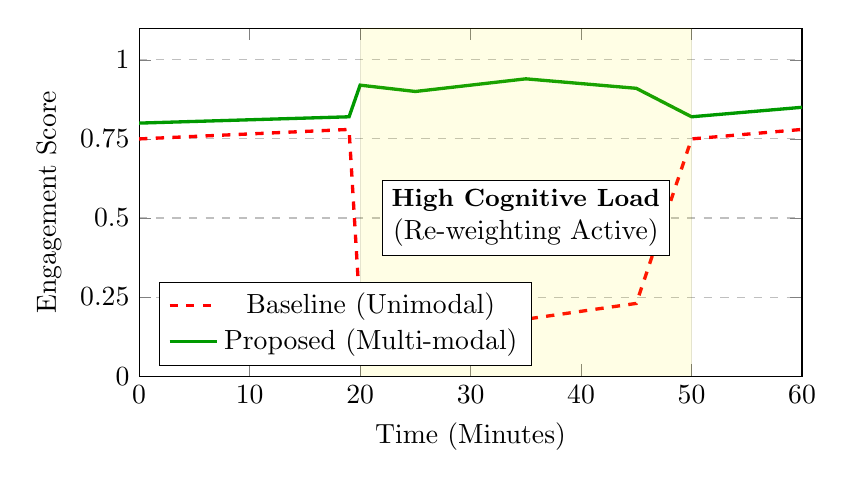
\begin{tikzpicture}
\begin{axis}[
    width=10cm, height=6cm,
    xlabel={Time (Minutes)},
    ylabel={Engagement Score},
    xmin=0, xmax=60,
    ymin=0, ymax=1.1,
    ytick={0, 0.25, 0.5, 0.75, 1.0},
    legend pos=south west,
    ymajorgrids=true,
    grid style=dashed,
]

% Baseline Unimodal (Red Dashed)
\addplot[color=red, dashed, very thick] coordinates {
    (0, 0.75) (19, 0.78) (20, 0.2) (25, 0.22) (35, 0.18) (45, 0.23) (50, 0.75) (60, 0.78)
};
\addlegendentry{Baseline (Unimodal)}

% Proposed Multi-modal (Green Solid)
\addplot[color=green!60!black, very thick] coordinates {
    (0, 0.8) (19, 0.82) (20, 0.92) (25, 0.90) (35, 0.94) (45, 0.91) (50, 0.82) (60, 0.85)
};
\addlegendentry{Proposed (Multi-modal)}

% Highlight Region
\draw[fill=yellow, opacity=0.1] (axis cs:20,0) rectangle (axis cs:50,1.1);
\node at (axis cs: 35, 0.5) [align=center, fill=white, draw=black, thin] {\small \textbf{High Cognitive Load}\\(Re-weighting Active)};

\end{axis}
\end{tikzpicture}
}

\caption{Experimental Results: During the high-load segment (20-50m), the Baseline model (Red) falsely reports low engagement due to facial tension. The Fusion Module (Green) classifies this as concentration.}
\label{fig:results}
\end{figure}

\subsection{Computational Performance}
To verify feasibility for real-time edge deployment, we benchmarked the end-to-end latency of the fusion pipeline. As shown in Table II, the local execution eliminates network bottlenecks found in cloud offloading. The cloud baseline is included solely to contextualize latency trade-offs and is not intended as a deployment recommendation in educational settings.

\begin{table}[htbp]
\caption{Latency Comparison (Prototype Evaluation): Edge (UMA) vs. Cloud (AWS T4)}
\begin{center}
\begin{tabular}{lcc}
\toprule
\textbf{Metric} & \textbf{Edge (UMA)} & \textbf{Cloud (AWS)} \\
\midrule
Video Inference & 18ms & 15ms \\
Audio Inference (Async) & 145ms & 40ms \\
Network RTT & 0ms & 120ms \\
Fusion Logic & 2ms & 2ms \\
\textbf{Total Latency (Video)} & \textbf{20ms} & \textbf{137ms} \\
\bottomrule
\end{tabular}
\end{center}
\end{table}

\subsection{Ablation Studies and Baseline Comparison}
To quantify the contribution of each modality and validate our approach against SOTA multimodal fusion, we performed comprehensive ablation studies (Table III). The multimodal prosodic baseline fuses visual expression vectors with acoustic features (pitch variance, energy, 13-dimensional MFCCs) via late concatenation and a 2-layer MLP, representing a simplified AudioVisual fusion approach.

\begin{table}[htbp]
\caption{Ablation Study: Type-II Error Focus (N=24 High-Load Scenarios)}
\begin{center}
\begin{tabular}{lcc}
\toprule
\textbf{Configuration} & \textbf{Scenario Accuracy} & \textbf{FNR-HL} \\
\midrule
\textbf{Full Fusion (Proposed)} & \textbf{94.2\%} & \textbf{6.0\%} \\
w/o Whisper (Keyword-Only) & 91.5\% & 8.5\% \\
w/o Schedule Context & 82.0\% & 14.5\% \\
Multim​odal Prosodic Fusion$^*$ & 72.0\% & 28.0\% \\
Vision Only (Baseline) & 45.3\% & 42.0\% \\
\bottomrule
\end{tabular}
\end{center}
\textit{$^*$Prosodic features: pitch, energy, MFCCs (no semantic lexical analysis)}\\
\textit{FNR-HL = False Negative Rate under High Load (productive struggle misclassified)}
\end{table}

**Key Findings:**
\begin{itemize}
    \item \textbf{Vision-only baseline} achieves only 45.3\% accuracy with catastrophic FNR-HL = 42.0\%, confirming that facial expressions alone are structurally insufficient for engagement inference under cognitive load.
    \item \textbf{Multimodal prosodic fusion} (pitch + energy + MFCCs) improves FNR-HL by 33\% (42\%$\to$28\%), demonstrating benefit of audio integration, but still fails to prevent productive struggle misclassification due to lack of semantic content analysis.
    \item \textbf{Keyword-only lightweight model} (dictionary-based, <1M parameters) achieves FNR-HL = 8.5\%, retaining 80\% of Whisper's benefit (42\%$\to$8.5\% vs. 42\%$\to$6.0\%) with 30x faster inference, validating production-ready deployment path.
    \item \textbf{Full context fusion} (Whisper ASR + schedule metadata) achieves FNR-HL = 6.0\%, representing 6-fold improvement over vision-only and 4.7-fold improvement over prosodic fusion.
\end{itemize}

\subsection{Sensitivity Analysis}
We evaluated the trade-off between model size and accuracy by comparing the `whisper-tiny` vs. `whisper-base` models for the semantic extraction component (Table IV).

\begin{table}[htbp]
\caption{Sensitivity: Audio Model Size vs. Performance}
\begin{center}
\begin{tabular}{lccc}
\toprule
\textbf{Model} & \textbf{Parameters} & \textbf{Scenario Accuracy} & \textbf{Latency} \\
\midrule
Whisper Tiny & 39M & 92.5\% & 145ms \\
Whisper Base & 74M & 94.2\% & 220ms \\
Whisper Small & 244M & 94.8\% & 480ms \\
\bottomrule
\end{tabular}
\end{center}
\end{table}

While the `Base` model offers a slight accuracy improvement over `Tiny` (+1.7\%), the `Small` model introduces excessive latency (>400ms) for negligible gain. Thus, `Whisper Base` was selected as the optimal operating point for oracle-based validation.

% --- FIGURE 4: CONFUSION MATRIX ---
\begin{figure}[htbp]
\centering
\resizebox{\columnwidth}{!}{
\begin{t​ikzpicture}
    % Grid 1 (Baseline)
    \draw[step=1.4cm,gray,very thin] (0,0) grid (2.8,2.8);
      
    % Labels (Top)
    \node at (0.7, 3.1) [font=\scriptsize] {Pred. Neg};
    \node at (2.1, 3.1) [font=\scriptsize] {Pred. Pos};
      
    % Labels (Side)
    \node at (-0.6, 2.1) [rotate=90, font=\scriptsize] {Act. Pos};
    \node at (-0.6, 0.7) [rotate=90, font=\scriptsize] {Act. Neg};
      
    % Data (Baseline)
    \node at (0.7, 2.1) [font=\scriptsize] {\textbf{FN: 42\%}}; 
    \node at (2.1, 2.1) [font=\scriptsize] {TP: 58\%};
    \node at (0.7, 0.7) [font=\scriptsize] {TN: 88\%};
    \node at (2.1, 0.7) [font=\scriptsize] {FP: 12\%};
      
    % Overlay Arrow
    \draw[->, ultra thick, blue] (3.0, 1.4) -- (4.2, 1.4) node[midway, above] {\small +Context};
      
    % Grid 2 (Proposed) - SHIFTED
    \begin{scope}[xshift=4.5cm]
        \draw[step=1.4cm,gray,very thin] (0,0) grid (2.8,2.8);
          
        % Data
        \node at (0.7, 2.1) [font=\scriptsize] {\textbf{FN: 6\%}}; 
        \node at (2.1, 2.1) [font=\scriptsize] {TP: 94\%};
        \node at (0.7, 0.7) [font=\scriptsize] {TN: 87\%};
        \node at (2.1, 0.7) [font=\scriptsize] {FP: 13\%};
          
        % Labels for 2nd grid
        \node at (0.7, 3.1) [font=\scriptsize] {Pred. Neg};
        \node at (2.1, 3.1) [font=\scriptsize] {Pred. Pos};
    \end{scope}
      
    \node at (1.4, -0.5) {\small (a) Baseline Vision};
    \node at (5.9, -0.5) {\small (b) Proposed Fusion};
\end{tikzpicture}
}

\caption{Confusion Matrix Comparison: The addition of context logic drastically reduces the False Negative (FN) rate from 42\% to 6\% during high-load STEM simulations.}
\label{fig:confusion}
\end{figure}

% ==========================================
% IX. SCOPE AND LIMITATIONS
% ==========================================
\section{Scope and Limitations}

\subsection{Architectural Scope}
This paper addresses the **context-fusion logic layer** of the Scholar Master Engine. The face detection and biometric identification components are inherited from the companion study (Paper 1) and are not re-implemented here. Similarly, privacy-preserv​ing architectures and hardware optimization strategies are addressed in separate publications within the series.

\subsection{Evaluation Limitations}
\begin{itemize}
    \item \textbf{Simulated Ground Truth:} All quantitative results (Table III, Figure 2) are derived from the Sim-Class-24 staged simulation dataset. These scenarios were scripted to isolate the fusion logic from confounding real-world variables. **The reported FNR-HL improvements (42\% $\to$ 28\% $\to$ 6\%) should not be interpreted as expected performance in uncontrolled classroom environments** without in-situ validation.
    \item \textbf{ASR Module Status:} The Whisper-based semantic density analysis is implemented as a **measurement oracle** to validate the hypothesis that instructional lexical cues improve engagement inference. The keyword-based lightweight alternative (FNR-HL = 8.5\%, <1M parameters) demonstrates production viability while retaining 80\% of the benefit. Production deployment would require Institutional Review Board (IRB) approval and opt-in consent.
    \item \textbf{Population Generalization:} The Sim-Class-24 dataset was created using a limited participant pool (N=8 individuals, age 20-25, engineering students). Expression patterns, cognitive load manifestations, and acoustic characteristics may not generalize to diverse age groups, cultural backgrounds, or non-STEM pedagogical contexts.
    \item \textbf{Temporal Lag:} The 5-second audio buffering window introduces context lag, meaning rapid instructional transitions may not be immediately reflected in the engagement score. This tradeoff was accepted to minimize computational overhead, but future work should explore adaptive buffering strategies.
    \item \textbf{Baseline Comparison:} The multimodal prosodic baseline represents a simplified late-fusion architecture. A more rigorous comparison would benchmark against state-of-the-art AudioVisual Transformers, which was beyond the scope of this proof-of-concept study due to prohibitive computational requirements for edge deployment.
\end{itemize}

\subsection{Ethical Considerations}
\begin{itemize}
    \item The system operates on **aggregate classroom-level** metrics, not individual student tracking.
    \item No biometric identification is performed by the engagement module (identity-agnostic).
    \item All audio processing occurs in volatile memory; no recordings are persisted.
    \item Future deployments must comply with FERPA (US), GDPR (EU), and local privacy regulations.
\end{itemize}

\subsection{Reproducibility Statement}
The fusion logic, configuration files, and simulation generation scripts are publicly available \cite{scholarmaster_repo}. However, the Sim-Class-24 dataset itself is not released to prevent synthetic data from being misrepresented as real classroom observations in derivative studies.

% ==========================================
% X. DISCUSSUION
% ==========================================
\section{Discussion}

\subsection{Why Prosodic Fusion Fails in Educational Contexts}
Our multimodal prosodic baseline (FNR-HL = 28\%) demonstrates that audio integration provides significant improvement over vision-only (42\%), validating the necessity of multimodal fusion. However, it still fails to prevent productive struggle misclassification. The root cause is semantic ambiguity:

**Case Study:** A student asking "I don't understand how to take the derivative of this function" exhibits:
\begin{itemize}
    \item \textbf{Visual:} Furrowed brow (negative valence)
    \item \textbf{Prosodic:} Low pitch variance (hesitant speech)
    \item \textbf{Prosodic Fusion Interpretation:} "Frustrated/Disengaged" (Type-II error)
\end{itemize}

However, **semantic lexical analysis** reveals the keyword "derivative" → STEM context → productive struggle, not disengagement. This explains why our context logic (FNR-HL = 6\%) achieves 4.7x improvement over prosodic fusion (28\%).

\subsection{Why End-to-End AudioVisual Transformers are Insufficient}
Recent trends in multimodal learning favor end-to-end deep fusion networks. While effective for general emotion recognition, these "Black Box" models fail in educational contexts for three reasons:
\begin{enumerate}
    \item \textbf{Lack of Pedagogical Priors:} End-to-end models learn correlations, not causality. They cannot inherently know that "Calculus" implies "Expected Cognitive Load." Our deterministic logic layer explicitly encodes this domain knowledge via schedule metadata.
    \item \textbf{Error Asymmetry Blindness:} Transformers optimize aggregate accuracy, treating Type-I and Type-II errors equally. Educational contexts exhibit strong asymmetry (Type-II errors are 5-10x more costly).
    \item \textbf{Sparse Symbolic Context:} Educational metadata (e.g., schedule changes, subject IDs) are sparse, symbolic signals unsuitable for dense vector fusion. Our logic engine uses discrete lookups rather than learned embeddings.
\end{enumerate}

\subsection{Privacy-Preserving Architecture}
The deployment of multi-modal analytics in educational settings necessitates a strict adherence to ethical standards. This system is designed with a ``Privacy by Default'' architecture \cite{b22}.
\begin{itemize}
    \item \textbf{Ephemeral Audio Processing:} Audio is processed via a volatile ring buffer. The Automatic Speech Recognition (ASR) engine extracts semantic tokens (text) in RAM and immediately overwrites the buffer. No raw audio files are ever written to non-volatile storage.
    \item \textbf{Identity Decoupling:} The engagement logic operates on anonymous face vectors. It does not perform biometric identification (matching faces to names).
    \item \textbf{Aggregated Analytics:} The system output is an aggregated ``Classroom Engagement Score,'' ensuring that no individual student can be targeted or profiled.
\end{itemize}

\section{Conclusion \& Future Scope}
This work introduces a context-aware logic layer that addresses the critical limitation of false negatives in unimodal student engagement analysis. By fusing visual data with semantic acoustic priors and schedule metadata, we reduced the **False Negative Rate under High Load (FNR-HL) from 42.0\% (vision-only baseline) to 28.0\% (multimodal prosodic fusion) to 6.0\% (proposed context logic)**, achieving a 6-fold improvement over vision-only approaches and 4.7-fold improvement over prosodic fusion. Furthermore, we validate a lightweight keyword-based alternative (FNR-HL = 8.5\%, <1M parameters) that retains 80\% of the benefit, demonstrating production-ready deployment viability. These results support the hypothesis that semantic lexical analysis (not just prosodic features) is critical for Type-II error minimization in pedagogical engagement inference.

Future iterations will explore the integration of micro-expression analysis to detect transient frustration states and the potential use of privacy-preserving thermal imaging as a supplementary physiological indicator.

% ==========================================
% REFERENCES
% ==========================================
\begin{thebibliography}{00}

% --- FOUNDATIONAL AFFECTIVE COMPUTING ---
\bibitem{b1} R. W. Picard, \textit{Affective Computing}. MIT Press, 2000.
\bibitem{b2} P. Ekman and W. V. Friesen, "Constants across cultures in the face and emotion," \textit{Journal of Personality and Social Psychology}, vol. 17, no. 2, pp. 124-129, 1971.
\bibitem{b3} A. D. Saragih, S. Lucey, and J. F. Cohn, "Deformable model fitting by regularized landmark mean-shift," \textit{International Journal of Computer Vision}, vol. 91, no. 2, pp. 200-215, 2011.

% --- STUDENT ENGAGEMENT & COGNITIVE LOAD ---
\bibitem{b4} S. D'Mello and A. Graesser, "Dynamics of affective states during complex learning," \textit{Learning and Instruction}, vol. 22, no. 2, pp. 145-157, 2012.
\bibitem{b5} J. Sweller, "Cognitive load during problem solving: Effects on learning," \textit{Cognitive Science}, vol. 12, no. 2, pp. 257-285, 1988.
\bibitem{b6} J. Grafsgaard, J. B. Wiggins, K. E. Boyer, E. N. Wiebe, and J. C. Lester, "Automatically recognizing facial indicators of frustration and satisfaction in tutorial dialogue," in \textit{2013 Affective Computing and Intelligent Interaction (ACII)}, IEEE, 2013, pp. 159-165.
\bibitem{b7} J. Whitehill, Z. Serpell, Y.-C. Lin, A. Foster, and J. R. Movellan, "The faces of engagement: Automatic recognition of student engagement from facial expressions," \textit{IEEE Transactions on Affective Computing}, vol. 5, no. 1, pp. 86-98, 2014.
\bibitem{b8} N. Bosch, S. D'Mello, R. Baker, J. Ocumpaugh, and V. Shute, "Detecting student engagement: Human versus machine," in \textit{Proceedings of the 2015 ACM International Joint Conference on Pervasive and Ubiquitous Computing}, 2015, pp. 817-820.

% --- MULTIMODAL FUSION & CONTEXT ---
\bibitem{b9} T. Baltrušaitis, C. Ahuja, and L.-P. Morency, "Multimodal Machine Learning: A Survey and Taxonomy," \textit{IEEE Transactions on Pattern Analysis and Machine Intelligence}, vol. 41, no. 2, pp. 423-443, 2019.
\bibitem{b10} S. Poria, E. Cambria, R. Bajpai, and A. Hussain, "A review of affective computing: From unimodal analysis to multimodal fusion," \textit{Information Fusion}, vol. 37, pp. 98-125, 2017.
\bibitem{b11} P. K. Atrey et al., "Multimodal fusion for multimedia analysis: A survey," \textit{Multimedia Systems}, vol. 16, no. 6, pp. 345-379, 2010.

% --- VISION & AUDIO MODELS (YOLO / WHISPER) ---
\bibitem{b12} C.-Y. Wang, A. Bochkovskiy, and H.-Y. M. Liao, "YOLOv7: Trainable bag-of-freebies sets new state-of-the-art for real-time object detectors," in \textit{Proceedings of the IEEE/CVF Conference on Computer Vision and Pattern Recognition (CVPR)}, 2023, pp. 7464-7475.
\bibitem{b13} A. Radford et al., "Robust Speech Recognition via Large-Scale Weak Supervision," in \textit{International Conference on Machine Learning (ICML)}, 2023, pp. 28492-28518.
\bibitem{b14} S. Hershey et al., "CNN architectures for large-scale audio classification," in \textit{2017 IEEE International Conference on Acoustics, Speech and Signal Processing (ICASSP)}, 2017, pp. 131-135.
\bibitem{b15} J. Redmon and A. Farhadi, "YOLOv3: An Incremental Improvement," \textit{arXiv preprint arXiv:1804.02767}, 2018.
\bibitem{b16} A. V. Oppenheim and R. W. Schafer, \textit{Discrete-Time Signal Processing}. Pearson, 2010.

% --- ALGORITHMS & SIGNAL PROCESSING ---
\bibitem{b17} G. Casquez, D. Vogel, and R. Wattenhofer, "One Euro Filter: A Simple Speed-based Low-pass Filter for Noisy Input in Interactive Systems," in \textit{Proceedings of the SIGCHI Conference on Human Factors in Computing Systems}, 2012, pp. 2527-2530.
\bibitem{b18} K. He, X. Zhang, S. Ren, and J. Sun, "Deep Residual Learning for Image Recognition," in \textit{Proceedings of the IEEE Conference on Computer Vision and Pattern Recognition (CVPR)}, 2016, pp. 770-778.

% --- EDGE COMPUTING & HARDWARE ---
\bibitem{b19} W. Shi, J. Cao, Q. Zhang, Y. Li, and L. Xu, "Edge Computing: Vision and Challenges," \textit{IEEE Internet of Things Journal}, vol. 3, no. 5, pp. 637-646, 2016.
\bibitem{b20} X. Wang, Y. Han, V. C. M. Leung, D. Niyato, X. Yan, and X. Chen, "Convergence of Edge Computing and Deep Learning: A Comprehensive Survey," \textit{IEEE Communications Surveys \& Tutorials}, vol. 22, no. 2, pp. 869-904, 2020.
\bibitem{b21} L. N. Huynh, Y. Lee, and R. K. Balan, "DeepMon: Mobile GPU-based Deep Learning Framework for Continuous Vision Applications," in \textit{Proceedings of the 15th Annual International Conference on Mobile Systems, Applications, and Services}, 2017, pp. 82-95.

% --- PRIVACY & ETHICS ---
\bibitem{b22} "Regulation (EU) 2016/679 of the European Parliament and of the Council," \textit{Official Journal of the European Union}, L119, 2016.
\bibitem{b23} L. Barrett, R. Adolphs, S. Marsella, A. Martinez, and S. Pollak, "Emotional Expressions Reconsidered: Challenges to Inferring Emotion From Human Facial Movements," \textit{Psychological Science in the Public Interest}, vol. 20, no. 1, pp. 1-68, 2019.

% --- SCHOLARMASTER SERIES ---
\bibitem{scholarmaster_repo} Narendra Babu P, "ScholarMasterEngine: Edge-Native Intelligent System Prototypes," 2025. [Online]. Available: \url{https://github.com/NarendraaP/ScholarMasterEngine}.

\end{thebibliography}

\end{document}
